\documentclass[pdflatex,sn-mathphys-num]{sn-jnl}

\usepackage{graphicx}%
\usepackage{multirow}%
\usepackage{amsmath,amssymb,amsfonts}%
\usepackage{amsthm}%
\usepackage{mathrsfs}%
\usepackage[title]{appendix}%
\usepackage{xcolor}%
\usepackage{textcomp}%
\usepackage{manyfoot}%
\usepackage{booktabs}%
\usepackage{algorithm}%
\usepackage{algorithmicx}%
\usepackage{algpseudocode}%
\usepackage{listings}%

\theoremstyle{thmstyleone}%
\newtheorem{theorem}{Theorem}%
\newtheorem{proposition}[theorem]{Proposition}%

\theoremstyle{thmstyletwo}%
\newtheorem{example}{Example}%
\newtheorem{remark}{Remark}%

\theoremstyle{thmstylethree}%
\newtheorem{definition}{Definition}%

\raggedbottom

\begin{document}

\title[LocalLLM-DataForge]{LocalLLM-DataForge: A Modular Framework for Synthetic User Story Decomposition with Local LLMs and LLM-as-a-Judge Evaluation}

\abstract{User story decomposition into development tasks is a common practice in agile projects that depends highly on human judgment. Attempts to automate this activity using machine learning techniques often face two recurring limitations: the scarcity of annotated datasets and the reliance on cloud-based language models. This work presents \textit{LocalLLM-DataForge}, a modular DataFrame-based framework for the generation and automated assessment of synthetic datasets aimed at user story decomposition using locally executed language models. The framework integrates generator and validator models within a reproducible pipeline, incorporating automatic validation mechanisms based on the \textit{LLM-as-a-Judge} paradigm and enabling experimentation with different model configurations and parameters. The proposal was evaluated on a dataset using multiple configurations of open-source models. The results show that it is possible to generate decompositions with consistent levels of quality, with notable differences in performance and stability depending on the model configuration. In particular, a trade-off between diversity and consistency is identified, associated with parameters such as temperature, as well as greater stability in structural criteria compared to higher variability in semantic criteria. These findings suggest that locally executed LLMs constitute a viable alternative for synthetic dataset generation in requirements engineering, providing advantages in terms of reproducibility, data control, and cost.}

\keywords{Requirements engineering, Natural language processing, Large language models,
Synthetic data generation, Task decomposition, Automated evaluation}

\maketitle

\section{Introduction}\label{sec1}

User stories are one of the most widely used requirement artifacts in agile software development. Teams commonly rely on them to capture functional needs from the end-user perspective in a concise and accessible manner \cite{cohn2004, beck2001}. In practice, their role extends beyond communication: user stories are routinely used to support planning, effort estimation, and day-to-day development activities. In particular, decomposing user stories into concrete development tasks is critical during backlog refinement and sprint planning \cite{rubin2012, schwaber2020}. Nevertheless, this activity still largely depends on manual work and the accumulated experience of the team.

When task decomposition is performed manually, a number of recurring issues tend to arise. Different team members may interpret the same user story in slightly different ways, leading to inconsistent levels of granularity and implicit assumptions that are never fully documented. Some relevant details may be overlooked (e.g., implicit functional constraints), while others may be excessively decomposed. Over time, these inconsistencies contribute to the creation of poorly structured backlogs, making estimation and task allocation more difficult \cite{lucassen2016}. The problem is often exacerbated in large or distributed teams, where the lack of shared decomposition practices weakens traceability and complicates the systematic automation of workflows in requirements engineering \cite{gorschek2006}.

Recent advances in Natural Language Processing (NLP), together with the rapid evolution of Large Language Models (LLMs), have opened new possibilities for automating tasks that have traditionally relied on software engineers \cite{chen2021, white2023}. Although previous works have explored the use of LLMs for requirements classification, ambiguity detection, test case generation, and the derivation of development tasks from natural language descriptions \cite{rahimi2023, sebban2024}, most of them depend on proprietary cloud-based models. This dependency introduces practical concerns related to cost, data confidentiality, reproducibility, and long-term availability, both in research and industrial contexts.

A common limitation among many LLM-based approaches is the lack of suitable datasets for training and evaluation. Public datasets specifically focused on user story decomposition remain scarce, largely due to the high cost of expert annotation and the sensitive nature of real-world requirements \cite{fucci2020}. The generation of synthetic data using LLMs has been proposed as a partial solution with limited visibility into how the generated results are validated. As a result, evaluating semantic correctness, completeness, and logical consistency becomes challenging \cite{liu2023}. Moreover, poorly controlled generation increases the risk of hallucinations, which can reduce confidence in the resulting datasets.

This work presents LocalLLM-DataForge, a modular framework designed to generate synthetic datasets for user story decomposition using locally executed LLMs. The framework leverages DataFrames to structure and manage intermediate results throughout the generation process. It also integrates with Ollama to run open-source language models without relying on cloud services. One of its core components is an intelligent caching mechanism, which avoids redundant computations during iterative experiments and helps reduce execution time when exploring different generation configurations.

Quality control is addressed through automatic validation mechanisms. LocalLLM-DataForge applies LLM-as-a-Judge strategies to score the generated task decompositions according to explicit quality criteria. Two evaluation approaches are considered. The first relies on a single generator and scores its outputs based on criteria such as coherence, completeness, feasibility, format, and granularity \cite{chiang2023}. The second compares outputs produced by multiple generators and selects the most appropriate decomposition. This comparative strategy leverages consensus-based principles that have been shown to improve reliability and reduce semantic errors in model outputs \cite{wang2023, li2024}.

This work makes two main contributions. First, it presents a fully local, extensible, and reproducible framework for generating synthetic datasets from user stories, explicitly addressing cost and privacy constraints. Second, it defines and operationalizes automatic validation strategies based on the LLM-as-a-Judge paradigm, adapted to requirements engineering artifacts.

To evaluate the feasibility of the proposed approach, experiments are conducted on the Salony\footnote{Salony: User Story Dataset available on Hugging Face, \url{https://huggingface.co/datasets/salony/User_story}.} dataset using several open-source LLMs. The results enable the analysis of both the quality of the generated decompositions and the behavior of comparative scoring strategies across models.

To evaluate the effectiveness and reliability of the proposed framework, this study is guided by the following research questions:

\textbf{RQ1:} How do variations in local LLM parameters, particularly temperature and model architecture, influence the balance between consistency and diversity in the generated user story decompositions?

\textbf{RQ2:} To what extent do structural and semantic evaluation criteria differ in terms of stability and agreement when applied through a local LLM-as-a-Judge paradigm?

\textbf{RQ3:} Is it feasible to achieve consistent and reliable evaluation scores using small-scale, locally hosted models in comparison with the expectations of traditional software engineering decomposition practices?

The remainder of this paper is organized as follows. Section~\ref{sec2} reviews related work on LLM-based automation in requirements engineering and synthetic data generation. Section~\ref{sec3} describes the architecture and main components of LocalLLM-DataForge. Section~\ref{sec4} presents the experimental setup and the obtained results. Section~\ref{sec5} discusses the findings and their implications, while Section~\ref{sec6} concludes the paper and outlines future work.

\section{Related Work}\label{sec2}

The automation of activities within requirements engineering has attracted increasing attention in recent years, particularly with the advancement of NLP techniques and, more recently, LLMs. Several studies have explored the potential of these models to support tasks traditionally considered challenging in natural language (e.g., elicitation, analysis, reformulation, and verification of requirements). Recent research shows that LLMs can improve the quality of requirements artifacts and facilitate the partial automation of various activities within the requirements engineering process, including user story generation, requirements classification, and textual quality evaluation \cite{hematt2025, zadenoori2025}. In particular, some works have demonstrated the feasibility of using LLMs to generate derived requirement artifacts or assist in their semantic analysis within software development workflows \cite{sami2024, proci2025}. These advances suggest that generative models can act as intelligent assistants in early stages of the software lifecycle, although their systematic integration into requirements engineering processes remains in an exploratory phase.

In parallel, synthetic data generation using generative models has emerged as a promising strategy to address the scarcity of annotated datasets across multiple domains. LLMs enable the production of large volumes of controlled textual data through prompt-based generation, facilitating the creation of datasets for training, evaluation, or augmentation of existing data. Recent studies have examined the use of LLMs for generating, curating, and evaluating synthetic data, highlighting their potential to complement or partially replace real datasets when these are limited or costly to obtain \cite{long2024}. Applications of this approach have been observed in various contexts, including the automatic generation of datasets in specialized domains such as digital forensics and AI-based legal systems \cite{fsidi2025, ma2025}. However, the literature also points out significant challenges related to the quality, coherence, and reliability of synthetically generated data, making it necessary to develop systematic validation and quality control mechanisms.

In this context, the \textit{LLM-as-a-Judge} paradigm has recently emerged, where language models are used not only as content generators but also as automatic evaluators of outputs produced by other models. This approach has been adopted in multiple studies on generative model evaluation, where LLMs act as evaluators capable of assessing complex semantic criteria that cannot be easily captured through traditional automatic metrics \cite{daly2025}. Recent research has shown that this type of evaluation can reasonably approximate human judgment in natural language generation tasks, particularly when explicit criteria or comparison-based evaluation schemes are used \cite{eigler2026}. Nevertheless, the use of LLMs as validators also introduces methodological challenges, including potential biases, prompt dependency, and risks of circularity when models evaluate each other.

Despite these advances, the current literature still presents a gap in the integration of these three research directions. In particular, there are few approaches that combine synthetic data generation, local model execution, and structured automatic evaluation and validation mechanisms within a single framework tailored to requirements engineering artifacts. LocalLLM-DataForge addresses this gap by proposing a framework designed to integrate these elements into an environment capable of systematically generating and evaluating user story decompositions.

\section{LocalLLM-DataForge Framework}\label{sec3}

LocalLLM-DataForge is a framework designed for the generation, transformation, and automated evaluation and validation of requirements engineering artifacts using locally executed language models. Its main purpose is to provide a modular, reproducible, and extensible architecture that enables the integration of multiple processing stages within a unified workflow.

Unlike traditional approaches focused on model training, LocalLLM-DataForge emphasizes the orchestration of pre-trained models for the controlled production of outputs and their systematic evaluation. This facilitates reproducible experimentation in environments without reliance on cloud-based services.

\subsection{General Architecture}

The framework is structured as a DataFrame-based processing pipeline, where each component represents an explicit transformation over the input data. This approach enables modeling the workflow as a sequence of deterministic and traceable operations, in which each stage produces new representations without modifying the original data. As a result, it promotes process auditability, intermediate result inspection, and experimental reproducibility.

The choice of a DataFrame-based model responds to the need to simultaneously manage multiple versions of generated artifacts. In particular, each user story may produce several decompositions generated by different models or configurations, which are stored as independent columns within the same structure. This organization enables systematic comparisons without requiring additional external structures or complex synchronization processes.

The overall pipeline follows five main stages: (1) data loading, (2) artifact generation, (3) comparison and evaluation, (4) metrics computation, and (5) results storage. These stages are not implemented as monolithic blocks, but rather as decoupled components operating over the same DataFrame. This design allows parts of the pipeline to be reorganized, extended, or replaced without affecting the rest of the framework.

A key aspect of the architecture is the explicit separation between generation and evaluation. While generator models are responsible for producing decompositions from user stories, the evaluation component operates independently to analyze the quality of these outputs, while a validation stage determines the acceptance or rejection of each instance based on the resulting scores under structured criteria. This separation enables experimentation with heterogeneous model configurations without introducing evaluation bias, and also facilitates the incorporation of new evaluation and validation mechanisms in future extensions of the framework.

Figure~\ref{fig:dataforge_architecture} illustrates the overall behavior of the pipeline modeled using a UML activity diagram, explicitly representing the processing flow and the parallel execution of generator models. The process begins with loading the user story dataset, followed by a parallel generation stage in which multiple models produce independent decompositions under different configurations. Subsequently, a validator component based on the \textit{LLM-as-a-Judge} paradigm compares the generated outputs, assigns evaluation scores, and determines validation outcomes. Finally, the results are integrated into the output DataFrame, enabling their systematic analysis.

This architectural design prioritizes modularity, transparency in data flow, and the ability to conduct controlled experimentation, which are essential aspects in studies aimed at evaluating the behavior of language models in requirements engineering tasks. Beyond simple orchestration, the framework provides explicit support for reproducible experimentation through structured dataflow modeling, integrated evaluation and validation mechanisms, and systematic management of multiple generated artifacts within a unified representation.

\begin{figure}[t]
\centering
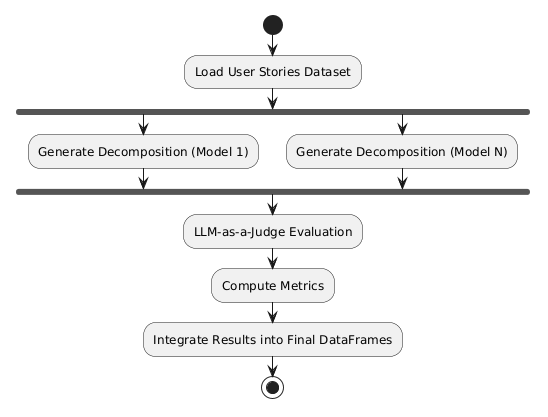
\includegraphics[width=\columnwidth]{images/diagram_en.png}
\caption{UML activity diagram of the LocalLLM-DataForge framework.}
\label{fig:dataforge_architecture}
\end{figure}

\subsection{Pipeline Execution Model}

The operational core of the framework is the \texttt{DataForgePipeline} class, which implements an execution model based on the sequential composition of modular steps. In this approach, each step is defined as a transformation function that receives an input DataFrame and produces an enriched DataFrame, preserving the original columns while adding new derived representations. This type of organization is consistent with dataflow-based processing models, where computation is expressed as a sequence of transformations over data \cite{dataflow_model}.

This model can be interpreted as a form of \textit{dataflow pipeline}, where the system state is explicitly materialized at each stage through tabular structures. Unlike traditional imperative architectures, in which transformations may overwrite previous information, the design adopted in LocalLLM-DataForge favors logical data immutability, enabling the traceability of the origin and evolution of each generated artifact throughout the process.

A distinctive feature of the pipeline is its declarative nature. Experiments are defined by specifying an ordered sequence of steps and their configurations, without the need to explicitly manage internal control flow. This approach contrasts with traditional practices based on ad-hoc scripts, which often hinder reproducibility and the reuse of experimental configurations. In this sense, recent frameworks for LLM-based data processing have highlighted the importance of modular abstractions and configurable pipelines to improve experiment traceability and reproducibility \cite{dataflow_llm}.

From an engineering perspective, this model promotes a high degree of decoupling between components. Each step encapsulates its processing logic and interacts with the rest of the pipeline exclusively through the shared DataFrame. This type of modular design has been widely adopted in modern data processing and machine learning systems, where the composition of reusable transformations enables the construction of complex workflows in a flexible manner \cite{dataflow_llm}.

Additionally, the pipeline supports incremental execution and intermediate result inspection. Since each transformation produces a new version of the DataFrame, it is possible to analyze the system state at any point in the workflow, which is particularly useful for debugging, prompt validation, and qualitative analysis of outputs generated by language models.

Overall, the pipeline model adopted in LocalLLM-DataForge provides a structured foundation for orchestrating LLMs in generation, evaluation, and validation tasks. In this way, it aligns with recent trends in the design of multi-stage LLM systems that integrate generative and evaluative components within a unified processing workflow \cite{llm_pipeline_eval}.

\subsection{Pipeline Components}

The framework incorporates a set of specialized components that encapsulate specific functionalities within the pipeline. This design follows principles of \textit{pipes-and-filters} architectures, in which processing is decomposed into a sequence of independent stages that progressively transform the input data. In this type of architecture, each component, or filter, performs a specific operation and passes its output to the next component through defined channels \cite{pipes_filters}. This approach has been widely adopted in data processing systems and machine learning pipelines, where the separation of concerns enables the construction of complex workflows from simple, decoupled transformations.

Within this scheme, the \texttt{LoadDataFrame} component acts as the entry point of the pipeline, handling the ingestion of structured data and its normalization into a unified tabular representation. Its role is to establish a consistent initial state that allows subsequent transformations to be applied without structural ambiguity. In turn, the \texttt{OllamaLLMStep} component encapsulates the interaction with locally executed language models, enabling the parameterization of their behavior through explicit configurations such as temperature, batch size, and maximum number of tokens. This component materializes model-generated outputs as new columns within the DataFrame, directly integrating the generated artifacts into the processing workflow. The incorporation of language models into structured pipelines reflects a recent trend in multi-stage systems, where multiple models collaborate to solve complex tasks through progressive information generation and transformation \cite{llm_multistage}.

The \texttt{ComparisonJudgeStep} component implements an evaluation mechanism based on the \textit{LLM-as-a-Judge} paradigm, in which a language model is used as an evaluator of outputs generated by other models. This approach has gained relevance as an alternative to traditional metrics in open-ended tasks, enabling the approximation of qualitative judgments through structured and reproducible scoring processes \cite{llm_judge_survey}. In this context, the component receives multiple generated candidates and produces quality scores that are directly integrated into the DataFrame, allowing for subsequent analysis without additional processing.

Together, these components form an architecture in which each stage of processing is clearly defined and decoupled, from generation to evaluation and validation. This separation of concerns not only enables the extension of the pipeline through the incorporation of new modules, but also supports experimentation with different model configurations and evaluation strategies without introducing rigid dependencies, aligning with fundamental design principles of data-oriented processing architectures.

\subsection{Local Execution and Resource Management}

A central feature of LocalLLM-DataForge is its focus on the local execution of language models, enabling full control over both the processed data and the computational resources used. Unlike cloud-based approaches, where inputs and outputs may be stored or processed by third parties, local execution ensures that all information remains within the user’s environment. This is particularly relevant in contexts involving sensitive data or subject to privacy regulations \cite{local_llm_privacy}. This aspect has been identified in the literature as one of the main advantages of open-source and locally deployed models, as it eliminates risks associated with data exposure and improves processing transparency \cite{local_llm_reproducibility}.

From an experimental perspective, local execution also contributes significantly to the reproducibility of results. In environments based on external APIs, factors such as changes in model versions, undocumented internal updates, or infrastructure variations may affect the obtained results. In contrast, using local models allows fixing specific versions, configurations, and execution conditions, ensuring that experiments can be replicated under identical settings \cite{local_llm_reproducibility}. This property is particularly important in studies aimed at evaluating the behavior of language models, where even minor environmental variations can significantly impact generated outputs.

However, local execution also introduces challenges related to efficient computational resource management. Language models require substantial memory and processing capacity, which necessitates mechanisms to optimize their use under hardware constraints. In this context, the framework implements a configurable batch processing scheme that controls the number of instances processed simultaneously, preventing context overflows and reducing memory pressure. This approach enables dynamic adaptation of pipeline execution to available hardware capabilities, maintaining a balance between performance and operational stability.

Additionally, an optional caching system is incorporated to reuse previously generated results when inputs and configurations remain unchanged. This strategy is particularly useful in iterative experimentation scenarios, where multiple executions with similar parameters are common. Reusing results not only reduces execution time but also contributes to experimental consistency by avoiding unnecessary variations in generated outputs.

Overall, the local execution approach adopted in LocalLLM-DataForge not only addresses privacy and data control considerations, but also represents a methodological choice aimed at ensuring reproducibility, traceability, and stability in the experimental process—key aspects for the rigorous experimental analysis of systems based on language models.

\subsection{Prompt Design}

Prompt design constitutes a central methodological component within the framework, as it defines how language models interpret tasks and generate their responses. In the context of LLMs, a prompt can be understood as a form of implicit programming, through which the behavior of the model can be guided without modifying its internal parameters \cite{prompt_survey}. Several studies have shown that the quality, structure, and clarity of prompts directly influence the accuracy, consistency, and usefulness of generated outputs, positioning prompt engineering as a key discipline for effectively leveraging these models \cite{prompt_engineering_review}.

In LocalLLM-DataForge, prompts are designed following a structured approach based on instruction–input–response schemas, where both content constraints and the expected output format are explicitly specified. This type of structuring has been identified as an effective strategy to improve result consistency and facilitate automatic processing, especially in tasks that require generating structured data \cite{structured_prompting}. In particular, enforcing rigid formats reduces ambiguity in outputs and enables their direct integration into the pipeline without requiring additional cleaning or normalization stages.

The framework employs two main prompts: (i) a \textit{task generation prompt}, responsible for decomposing user stories into structured sets of tasks, and (ii) an \textit{evaluation prompt under the LLM-as-a-Judge approach}, aimed at assessing the quality of such decompositions according to defined criteria.

The \textit{generation prompt} follows an instruction–input–response scheme, explicitly specifying decomposition constraints such as non-overlapping tasks, clarity in phrasing, and the requirement of a structured format based on summary and description fields. These constraints delimit the model’s output space, promoting the generation of consistent and comparable artifacts.

The \textit{evaluation prompt}, in turn, instructs the model to compare two alternative decompositions of the same user story and produce a structured judgment. The evaluation is based on five quality criteria and outputs a JSON-formatted response that includes numerical scores and a final decision indicating the preferred alternative.

Both prompts are designed under homogeneous principles of structure and control, while serving distinct functional objectives within the pipeline. To ensure experimental reproducibility and methodological transparency, the complete versions of these prompts are provided in Appendix~\ref{appendix:task_generation_prompt} and Appendix~\ref{appendix:llm_judge_prompt}, respectively.

In generation tasks, the prompt is specifically designed to produce user story decompositions under defined constraints, such as non-overlapping tasks, clarity in wording, and the inclusion of structured fields like summary and description. These constraints act as control mechanisms that bound the model’s output space, favoring the production of consistent and comparable artifacts. In evaluation and validation tasks, the LLM-as-a-Judge prompt explicitly defines quality criteria and decision rules, instructing the model to produce structured judgments in formats such as JSON. This approach enables the transformation of qualitative assessments into quantifiable representations that can be directly integrated into the processing pipeline.

Additionally, the use of standardized prompts across different models enables fairer and more controlled comparisons, avoiding biases introduced by model-specific prompt tuning. Recent literature has highlighted that consistency in prompt design is a critical factor for ensuring the validity of comparative evaluations across LLMs, as even minor variations in phrasing can significantly impact the results \cite{structured_prompting}. In this sense, the framework adopts a uniform approach to prompt definition, ensuring that observed differences in outputs are primarily attributable to model characteristics rather than variations in instructions.

For this reason, prompt design in LocalLLM-DataForge is not merely a configuration task, but a fundamental element of the experimental process, acting as the control interface between the researcher and the model. This perspective aligns with recent trends that consider prompt engineering as a key abstraction layer in systems based on language models.

\section{Results}\label{sec4}

This section presents the results of the experimental study conducted to evaluate the performance of the proposed \textit{framework} in the automatic generation of user story decompositions. First, the experimental setup is described, including the execution environment, the models used, and the evaluation scheme. Next, the aggregated results obtained across the different tests are presented, followed by a detailed criterion-level analysis that allows the identification of behavioral patterns and differences between models. Finally, the most relevant findings derived from the study are discussed.

\subsection{Experimental Setup}

The experimental study was conducted using the \textit{LocalLLM-DataForge} framework, aimed at evaluating the automated generation of user story decompositions through locally deployed LLMs.

The hardware environment consisted of a Dell server equipped with an AMD EPYC 9124 processor at 3.0 GHz (16 cores, 32 threads, 64 MB cache), 64 GB of DDR5-4800 RAM (4 $\times$ 16 GB modules), and an NVIDIA Ampere A2 GPU with 16 GB of VRAM. The pipeline was implemented using Python v3.13.7, with Ollama v0.21.2 serving as the orchestration platform for local model execution. The GPU was utilized to accelerate model inference, thereby reducing generation and evaluation times during the experimental trials.

The primary dataset was Salony, from which 1,139 out of 1,998 user stories were selected based on their adherence to the canonical structure: \textit{“As a(n) [role], I want [feature] so that [benefit]”}. Each story was processed by two generator models (G1 and G2), configured with distinct temperature settings. Specifically, G1 operated at a temperature of 0.3 to favor deterministic outputs, whereas G2 was set to 0.7 to promote output diversity. The judge model utilized a temperature of 0.2 to ensure consistency in its evaluative judgments.

The generated decompositions were assessed using an \textit{LLM-as-a-Judge} paradigm, assigning scores across five criteria: coherence, completeness, feasibility, format, and granularity \cite{llm_judge_frontiers_2025}. 

In this work, it is important to distinguish between evaluation and validation. Evaluation refers to the scoring process performed by the \textit{LLM-as-a-Judge} across the defined quality criteria. In contrast, validation refers to the framework's capacity to accept or reject a generated decomposition based on those scores, according to a predefined threshold. This distinction ensures a clear separation between the assessment of quality and the decision-making process derived from it.

The selection of these criteria is grounded in the requirements quality principles established by the ISO/IEC/IEEE 29148:2018 standard \cite{iso29148}. In this context, coherence assesses semantic correspondence with the user story; completeness measures the degree of requirement coverage; feasibility evaluates the technical viability of the tasks; format examines the clarity and structure of the output; and granularity determines the appropriateness of the decomposition level.

Each criterion was evaluated on a scale from 0 to 10, resulting in a maximum possible score of 50 points \cite{likert5to7range}. The total score for each instance was calculated as the sum of the five criteria. Based on these scores, a passing threshold of 35 points (70\%) was established to classify each instance as either valid or invalid \cite{threshold70}.

Aggregate metrics, including the mean and standard deviation of total scores, were calculated for the evaluated set. The pass rate was defined as the percentage of instances exceeding the established threshold, representing the validation outcome of the framework. Furthermore, the win rate was calculated through head-to-head comparisons between two decompositions, representing the percentage of instances in which one decomposition was preferred over another based on the evaluation scores assigned by the judge model. This metric reflects comparative evaluation rather than threshold-based validation.

To analyze the impact of different LLM configurations, four experimental setups (C1, C2, C3, and C4) were defined. Each configuration comprised two generator models (G1 and G2) and one \textit{LLM-as-a-Judge} evaluator. The evaluated configurations, presented in Table~\ref{tab:model_configs}, include models from various families, sizes, and architectures.

\begin{table}[ht]
\centering
\caption{Model configurations evaluated in experimental tests}
\label{tab:model_configs}
\begin{tabular}{lcccc}
\toprule
Config. & Role & Model & Architecture & Size \\
\midrule
\multirow{3}{*}{C1}  
& G1 & Llama 3.1 & Dense Transformer (decoder) with GQA & 8B \\
& G2 & Mistral & Transformer with Sliding Window Attention & 7B \\
& Judge & Qwen 3 & Hybrid Transformer with GQA \& Reasoning Mode & 14B \\
\midrule
\multirow{3}{*}{C2}  
& G1 & Qwen 3 & Hybrid Transformer with GQA \& Reasoning Mode & 8B \\
& G2 & Gemma 4 (E4B) & Efficient Transformer with PLE & 4B \\
& Judge & Qwen 2.5 & Dense Transformer with SwiGLU \& GQA & 14B \\
\midrule
\multirow{3}{*}{C3}  
& G1 & Gemma 3 & Multimodal Transformer with QK Norm & 12B \\
& G2 & Mistral Nemo & Dense Transformer (decoder) with GQA & 12B \\
& Judge & Qwen 3 & Hybrid Transformer with GQA \& Reasoning Mode & 14B \\
\midrule
\multirow{3}{*}{C4}  
& G1 & Qwen 3 & Hybrid Transformer with GQA \& Reasoning Mode & 14B \\
& G2 & Phi-4 & Dense Transformer (10T synthetic data tokens) & 14B \\
& Judge & GPT-OSS & Sparse MoE (3.6B active) with Variable CoT & 20B \\
\bottomrule
\end{tabular}
\end{table}

In each configuration, both generators processed the same set of user stories, producing alternative decompositions for each instance. This ensures input consistency across models and facilitates a direct comparison of their outputs. Subsequently, the judge model analyzed both decompositions and assigned evaluation scores based on the five quality criteria and performed a comparative selection to determine a preferred decomposition for each case.

\subsection{Global Results}

To identify consistent patterns in the behavior of the LLM-as-a-Judge evaluation model, a comparative analysis was conducted by aggregating the results of the experimental tests. This approach enables the observation of global trends regarding performance, stability, and relative behavior between models.

Table~\ref{tab:global_results} presents the aggregate metrics for each configuration, including the average score with its corresponding standard deviation (\textit{Mean} $\pm$ \textit{Std}), as well as the pass rate (\textit{Pass}) and the win rate in head-to-head comparisons (\textit{Win}).

\begin{table}[ht]
\centering
\caption{Aggregate results per experimental test}
\label{tab:global_results}
\begin{tabular}{cllccc}
\toprule
Config. & Generator & Mean $\pm$ Std & Pass (\%) & Win (\%) \\
\midrule
C1 & G1: Llama 3.1 & $24.21 \pm 21.86$ & 55.14 & 72.78 \\
C1 & G2: Mistral & $24.46 \pm 22.13$ & 55.31 & 27.22 \\
\midrule
C2 & G1: Qwen 3 & $39.74 \pm 5.29$ & 94.91 & 18.70 \\
C2 & G2: Gemma 4 & $42.23 \pm 2.89$ & 99.56 & 81.30 \\
\midrule
C3 & G1: Gemma 3 & $43.51 \pm 13.88$ & 90.87 & 99.56 \\
C3 & G2: Mistral Nemo & $34.39 \pm 11.15$ & 83.93 & 0.44 \\
\midrule
C4 & G1: Qwen 3 & $31.50 \pm 18.33$ & 73.22 & 54.96 \\
C4 & G2: Phi 4 & $32.34 \pm 18.39$ & 75.33 & 45.04 \\
\bottomrule
\end{tabular}
\end{table}

Overall, model behavior varies significantly across configurations, with notable differences in both performance and stability. However, the interpretation of mean scores requires careful consideration due to the presence of skewed distributions.

In particular, low mean values observed in configurations such as C1 and C4 are strongly influenced by the occurrence of zero-score instances. Prior to aggregation, a data cleaning and normalization step was performed to correct formatting inconsistencies in the outputs of the LLM-as-a-Judge, ensuring that all evaluation scores were properly parsed and aligned across criteria. After this process, zero-score values were preserved as valid outcomes, corresponding to cases where the generated decompositions were assigned the lowest possible evaluation score. As a result, the score distributions remain highly skewed, with a substantial gap between mean and median values.

This effect is especially evident in C1, where both generators exhibit similar mean scores despite the boxplot in Figure~\ref{fig:global_boxplot} showing relatively high median values. This indicates that while models such as Llama 3.1 and Mistral are capable of producing high-quality outputs, they also frequently generate decompositions that receive low evaluation scores and are subsequently classified as invalid under the validation threshold.

In contrast, C2 presents a more stable scenario, with higher mean scores and lower standard deviation. The tighter distribution suggests more consistent performance, particularly for Gemma 4, which outperforms Qwen 3 across all reported metrics.

C3 exhibits the clearest separation between generators, where Gemma 3 achieves both higher scores and a more concentrated distribution compared to Mistral Nemo. This indicates not only better average performance but also greater reliability in the generated outputs.

C4, on the other hand, represents a high-variance scenario rather than true convergence. Although both generators (Qwen 3 and Phi 4) show similar mean values, the distribution reveals wide dispersion and multiple zero-score instances, indicating unstable behavior and inconsistent output quality.

Figure~\ref{fig:global_boxplot} further illustrates these patterns by showing the full distribution of scores across configurations.

\begin{figure}[ht]
\centering

\includegraphics[width=\columnwidth]{images/total_score_distribution.png}
\caption{Distribution of total scores by configuration for generators with low temperature (G1: T=0.3) and high temperature (G2: T=0.7).}
\label{fig:global_boxplot}
\end{figure}

The discrepancy between mean values and medians observed in several configurations highlights the limitations of relying solely on average-based metrics. In skewed distributions, a high median combined with a low mean indicates the presence of frequent failure cases that significantly impact overall performance.

From a distributional perspective, configurations such as C1 and C4 exhibit large variability and a high number of low-score outliers, reflecting instability in generation quality. In contrast, configurations like C2 show tighter score distributions, suggesting more reliable and consistent behavior.

These findings underscore the importance of considering both central tendency and variability when evaluating model performance. From an engineering standpoint, reliability becomes a critical factor: a model that occasionally produces high-quality outputs but frequently frequently fails validation under the established threshold.

\subsection{Criterion-based Analysis}

The disaggregated analysis by criterion enables a more detailed understanding of model behavior beyond aggregate metrics. Table~\ref{tab:global_criteria} presents the average scores per evaluation criterion for each configuration. Additionally, Figure~\ref{fig:global_criteria_plot} illustrates the comparison across the five evaluation criteria for each configuration and generator.

\begin{table}[ht]
\centering
\caption{Average scores per criterion across the configurations and generators.}
\label{tab:global_criteria}
\begin{tabular}{clccccc}
\toprule
Config. & Generator  & Coherence & Completeness & Feasibility & Format & Granularity \\
\midrule
C1 & G1: Llama 3.1 & 4.92 & 4.58 & 4.97 & 5.27 & 4.48 \\
C1 & G2: Mistral & 4.79 & 4.88 & 4.94 & 5.27 & 4.57 \\
\midrule
C2 & G1: Qwen 3 & 8.60 & 7.81 & 7.82 & 8.86 & 6.64 \\
C2 & G2: Gemma 4 & 8.72 & 9.33 & 8.16 & 8.97 & 7.06 \\
\midrule
C3 & G1: Gemma 3 & 8.63 & 8.98 & 8.45 & 8.97 & 8.46 \\
C3 & G2: Mistral Nemo & 7.19 & 6.13 & 7.27 & 7.58 & 6.21 \\
\midrule
C4 & G1: Qwen 3 & 6.53 & 5.89 & 6.60 & 6.64 & 5.85 \\
C4 & G2: Phi 4 & 6.44 & 6.63 & 6.43 & 6.64 & 6.20 \\
\bottomrule
\end{tabular}
\end{table}


\begin{figure}[ht]
\centering

\includegraphics[width=\columnwidth]{images/criterion_comparison_all.png}
\caption{Comparison of criteria by configuration and generator.}
\label{fig:global_criteria_plot}
\end{figure}

Overall, the results reveal that performance varies not only across configurations but also across evaluation criteria, with no single model consistently outperforming the other in all dimensions.

The \textit{coherence} criterion exhibits relatively stable behavior across configurations, with both generators achieving similar scores and only minor variations. This suggests that maintaining logical consistency in the generated decompositions is less sensitive to model or configuration changes.

In contrast, \textit{completeness} shows more variability. In C2, Gemma 4 clearly outperforms Qwen 3, indicating stronger coverage of requirements. However, this trend reverses in C3, where Gemma 3 achieves significantly higher scores. This pattern suggests that completeness is highly dependent on the interaction between model and configuration.

For \textit{feasibility}, both models perform comparably in simpler configurations such as C1 and C2. However, in C3, Gemma 3 achieves higher scores, indicating better alignment with implementable task decomposition. Differences in C4 are less pronounced, reflecting a more balanced behavior.

The \textit{format} criterion remains one of the most stable across all configurations. Both generators achieve nearly identical scores in C1, C2, and C4, suggesting that adherence to structural formatting constraints is largely independent of the model. A noticeable difference appears only in C3, where Gemma 3 outperforms Mistral Nemo.

Finally, \textit{granularity} reveals more significant variation. While differences are minor in C1 and C4, C3 again shows a clear advantage for Gemma 3, indicating a more appropriate level of task decomposition. In C2, Gemma 4 exhibits slightly better performance, although the difference is less pronounced than in C3.

It is important to note that these criterion-level averages are also influenced by the presence of zero-score instances discussed in the previous section. Outputs assigned very low evaluation scores across all criteria contribute to lower averages, thereby affecting the overall averages and reinforcing the need to interpret these results in conjunction with distribution-based analyses.

Overall, the findings indicate that model performance is highly configuration-dependent and varies across evaluation dimensions. Rather than exhibiting consistent superiority, each model demonstrates strengths under specific conditions. In particular, differences become more pronounced in complex configurations such as C3, where both performance level and variability across criteria increase.

\section{Discussion}\label{sec5}

The results obtained enable an analysis not only of model performance but also of the implications of using local LLMs within structured pipelines for generating requirements engineering artifacts.

In particular, the discussion is structured around the research questions introduced in Section~\ref{sec1}, addressing the impact of model configuration (RQ1), the stability of evaluation criteria (RQ2), and the feasibility of using locally hosted models for reliable validation (RQ3).

This behavior is consistent with recent literature on the application of LLMs in requirements engineering. Studies such as \cite{zadenoori2025} indicate that performance in natural language processing tasks is highly dependent on factors such as prompt design, generation configuration, and usage context. Similarly, Norheim et al. \cite{sami2024} identify configuration sensitivity as a central challenge, aligning with the variations observed between configurations C2 and C3 in this study.

Overall, model performance is non-uniform and strongly dependent on the experimental setup. The differences observed between configurations such as C2 and C3 suggest that factors such as model selection, parameterization, and interaction within the pipeline significantly influence the quality of generated decompositions. This reinforces the idea that model selection cannot be treated in isolation but rather as part of a joint configuration problem involving both generators and LLM-as-a-Judge evaluation models.

In response to \textbf{RQ1}, the results indicate that variations in model configuration, particularly temperature and model architecture, significantly affect the balance between consistency and diversity in generated decompositions. Configurations such as C2 and C3 illustrate this trade-off, where higher variability is associated with increased diversity but reduced stability, while more controlled settings favor consistent but potentially less diverse outputs.

Configuration C4 provides a particularly relevant scenario in which generators operate under more comparable capacity conditions. In this context, performance differences are reduced, suggesting that part of the variability observed in other configurations may be associated not only with parameters such as temperature but also with differences in model capacity and architecture. When these factors are more controlled, performance tends to converge, and differences become more subtle, relating to generation style or prioritization of quality criteria.

A key observation concerns the difference between generators G1 and G2 in terms of stability and variability. This phenomenon has been reported in prior work. Niv \cite{hematt2025} notes that LLMs can achieve high average performance while exhibiting significant variability across executions. In this study, G2 occasionally achieves higher average scores (e.g., in C2), but with greater dispersion, indicating less consistent output quality. In contrast, G1 tends to produce more stable results, particularly in more complex configurations such as C3.

This behavior can be partially explained by the temperature parameter used during generation. Lower temperatures favor more deterministic outputs and improved consistency, while higher temperatures introduce diversity at the cost of increased variability \cite{li2026temp}. This directly supports the observations associated with RQ1. However, this relationship is task-dependent, highlighting the importance of careful parameter calibration within generation pipelines.

From the perspective of evaluation criteria, the results suggest a distinction between structural and semantic dimensions of quality. Criteria such as \textit{format} and \textit{coherence} exhibit relatively stable behavior across configurations, indicating that LLMs can reliably adhere to structural constraints when these are explicitly defined. In contrast, criteria such as \textit{completeness} and \textit{granularity} show greater variability, reflecting the increased difficulty of capturing deeper semantic aspects of task decomposition.

An additional factor influencing these results is the presence of zero-score evaluations, which persist even after applying data cleaning and normalization procedures to correct formatting inconsistencies in LLM-as-a-Judge outputs. These cases do not arise from parsing errors but reflect extremely low evaluation scores assigned by the LLM-as-a-Judge model. This behavior may be attributed to several factors: limitations of locally hosted models in handling complex evaluation prompts, sensitivity to parameter configurations (e.g., temperature), and the inherent difficulty of assessing semantically rich criteria such as completeness and granularity. Additionally, prompt design may play a role, as overly strict or ambiguous evaluation instructions can increase the likelihood of full rejection. This suggests that zero-score instances are not merely artifacts but an important signal of the interaction between model capacity, evaluation criteria complexity, and prompt formulation.

With respect to \textbf{RQ2}, these results indicate that the observed differences between structural and semantic criteria translate into distinct levels of evaluation reliability. While structural aspects can be assessed with relatively high consistency, semantic properties introduce greater variability, suggesting inherent limitations of LLM-as-a-Judge approaches when dealing with deeper requirement understanding.

This observation aligns with findings reported by Ferrari and Spoletini \cite{proci2025}, who note that LLMs perform well in tasks involving formal constraints but face challenges in aspects requiring deeper semantic understanding, such as requirement coverage. These limitations help explain the higher stability observed in structural criteria compared to semantic ones.

In particular, \textit{completeness} emerges as one of the most configuration-sensitive criteria. While G2 performs better in C2, its performance decreases in more complex scenarios such as C3, suggesting that requirement coverage depends not only on generative capacity but also on the ability to maintain semantic consistency as task complexity increases.

Similarly, \textit{granularity} plays a key role in differentiating model behavior. The results observed in C3 indicate that certain models are better able to balance the level of detail in task decomposition, avoiding both excessive fragmentation and overly coarse outputs. This aspect is particularly relevant in agile planning contexts, where decomposition quality directly impacts estimation and execution.

Another relevant finding is the effectiveness of the \textit{LLM-as-a-Judge} approach. Using an evaluation model to compare alternative decompositions enables the identification of qualitative differences that are not captured by aggregate metrics alone. In this context, the win rate serves as a complementary indicator of relative preference.

This approach is consistent with recent research advocating the use of LLMs as automated validators \cite{eigler2026}. While these systems can achieve performance comparable to human evaluators, they also present limitations, including potential biases and variability in scoring. In this study, configuration differences suggest that parameters such as temperature influence not only generation but also evaluation stability. Approaches such as \cite{daly2025} propose combining automated evaluation with iterative refinement and human validation to improve reliability.

Regarding synthetic data generation, the results are consistent with studies such as \cite{long2024}, which indicate that LLMs can produce high-quality synthetic data, albeit with limitations in consistency and coverage. Similarly, \cite{ma2025, fsidi2025} highlight the importance of robust validation mechanisms when using synthetic data in domain-specific applications. These findings are reflected in this study, where decomposition quality depends strongly on both configuration and evaluation processes.

From a practical perspective, the results suggest that local LLMs constitute a viable alternative for generating synthetic datasets in requirements engineering, provided that structured validation mechanisms are incorporated into the pipeline. While controlled generation combined with automated evaluation can mitigate variability, the results also indicate that output quality remains highly configuration-dependent. Therefore, these systems should be considered as support tools rather than replacements for human validation.

Regarding \textbf{RQ3}, the results demonstrate that locally hosted models can achieve consistent and practically usable outcomes derived from evaluation scores and validation thresholds, particularly under controlled configurations. While performance may not fully match that of large-scale proprietary systems, the observed results indicate that local LLMs are capable of supporting decomposition and evaluation tasks with acceptable levels of reliability, especially when combined with structured pipelines and validation strategies.

Overall, the results provide coherent answers to the proposed research questions, emphasizing the importance of configuration design (RQ1), the differentiated behavior of evaluation criteria (RQ2), and the practical viability of local LLM-based approaches (RQ3) within requirements engineering workflows.

This study also presents several limitations. In terms of internal validity, the use of an LLM-as-a-Judge raises questions about whether the evaluation reflects actual decomposition quality or is influenced by the characteristics of the validator model. Although explicit criteria and conservative configurations were used, potential biases cannot be fully eliminated.

Regarding construct validity, while the selected criteria (coherence, completeness, feasibility, format, and granularity) are grounded in the literature, they may not capture all relevant aspects of decomposition quality, such as traceability or alignment with business objectives.

In terms of external validity, the experiments were conducted using a single dataset (Salony), which limits the generalizability of the results. The relatively homogeneous structure of the user stories may also favor model performance compared to more diverse or unstructured datasets.

Finally, these results open several directions for future work, including the incorporation of hybrid evaluation strategies combining automated and human validation, the exploration of consensus mechanisms among multiple evaluators, and the extension of the framework to other types of requirements artifacts. Additionally, further research could analyze the impact of advanced prompting techniques and fine-tuning strategies on decomposition quality.

\section{Conclusion}\label{sec6}

This paper presented \textit{LocalLLM-DataForge}, a modular framework for the automated generation and validation of user story decompositions using locally executed large language models. The proposed approach addresses two key challenges in requirements engineering: the scarcity of annotated datasets and the dependence on cloud-based LLM services. By leveraging a DataFrame-driven pipeline architecture, the framework enables reproducible and controlled experimentation, integrating both generation and validation processes within a unified workflow.

The results provide clear answers to the research questions guiding this study. Regarding \textbf{RQ1}, the findings demonstrate that model configuration—particularly temperature and model architecture—has a significant impact on the balance between consistency and diversity in generated decompositions. While some configurations favor higher average performance, they may also introduce increased variability, highlighting the need for careful calibration within generation pipelines.

In relation to \textbf{RQ2}, the results show that evaluation criteria exhibit different levels of stability. Structural aspects such as \textit{format} and \textit{coherence} can be assessed with high consistency, whereas semantic dimensions such as \textit{completeness} and \textit{granularity} remain more variable and challenging to evaluate. This suggests inherent limitations of current LLM-as-a-Judge approaches when dealing with deeper semantic properties of requirements artifacts.

Concerning \textbf{RQ3}, the findings indicate that locally hosted models can achieve consistent and practically usable validation outcomes when integrated into structured pipelines. Although performance may not fully match that of large-scale proprietary systems, the results support the feasibility of local LLM-based approaches as a viable alternative for both generation and evaluation tasks in requirements engineering.

Overall, this work demonstrates that local LLM-based pipelines constitute a practical and reproducible approach for synthetic dataset generation. Beyond reducing dependency on external services, the proposed framework enables systematic experimentation and controlled evaluation, contributing to greater transparency in LLM-based research.

The main contributions of this work are twofold: (i) the design and implementation of a fully local and extensible framework for synthetic data generation from user stories, explicitly addressing cost and privacy constraints; and (ii) the integration and empirical evaluation of automated evaluation and validation mechanisms based on the \textit{LLM-as-a-Judge} paradigm within reproducible experimental pipelines, providing insights into the impact of configuration on both performance and stability.

Future work will focus on improving evaluation reliability through hybrid approaches that combine automated and human validation, as well as exploring consensus mechanisms among multiple LLM-as-a-Judge evaluation models to mitigate bias. Additionally, extending the dataset to more diverse and less structured domains will be essential to assess the generalizability of the approach. Further research will also investigate the impact of advanced prompting techniques and fine-tuning strategies, as well as the application of the framework to other requirements engineering artifacts such as use cases and functional specifications.

\backmatter

\begin{appendices}

\section{Task Generation Prompt}
\label{appendix:task_generation_prompt}

\begin{lstlisting}[basicstyle=\ttfamily\small, breaklines=true, caption={Prompt for Task Generation}, label={lst:task_generation_prompt}]
Below is an instruction that describes a task, paired with an input that provides a user story.

Write a response that appropriately completes the request.

Instruction:

Break this user story into smaller development tasks to help the developers implement it efficiently. You can divide this user story into as many tasks as needed, depending on its complexity. Each task must be unique, actionable, and non-overlapping.

Use the following format for the response:

1. summary: <task summary 1>
description: <task description 1>
2. summary: <task summary 2>
description: <task description 2>

N. summary: <task summary N>
description: <task description N>

Input:

{user_story}

Response:
\end{lstlisting}

\section{LLM-as-a-Judge Evaluation Prompt}
\label{appendix:llm_judge_prompt}

\begin{lstlisting}[basicstyle=\ttfamily\small, breaklines=true, caption={LLM-as-a-Judge Prompt}, label={lst:llm_judge_prompt}]
You are an expert software development manager evaluating two different breakdowns of a user story into development tasks.

Your job is to compare both breakdowns and determine which one is better overall.

USER STORY:
{user_story}

BREAKDOWN A:
{tasks_a}

BREAKDOWN B:
{tasks_b}

Evaluate both breakdowns based on these criteria (0-10 points each), aligned with ISO/IEC/IEEE 29148:2018 quality standards:

1. COHERENCE: Semantic correspondence between the generated tasks and the original user story. Does it maintain consistency with the user story intent? (0-10)
2. COMPLETENESS: Degree of coverage of implicit and explicit requirements. Does it cover all necessary aspects of the user story? (0-10)
3. FEASIBILITY: Technical feasibility of the proposed tasks. Are the tasks realistically implementable? (0-10)
4. FORMAT: Structure and clarity of the output. Is the response well-formatted, unambiguous, and easy to understand? (0-10)
5. GRANULARITY: Appropriateness of the decomposition level. Are tasks properly sized (not too big, not too small) and atomic? (0-10)

Respond in this exact JSON format:
{
  "breakdown_a": {
    "coherence": [score_0_to_10],
    "completeness": [score_0_to_10],
    "feasibility": [score_0_to_10],
    "format": [score_0_to_10],
    "granularity": [score_0_to_10],
    "total_score": [sum_of_all_scores],
    "strengths": "[brief_description_of_strengths]",
    "weaknesses": "[brief_description_of_weaknesses]"
  },
  "breakdown_b": {
    "coherence": [score_0_to_10],
    "completeness": [score_0_to_10],
    "feasibility": [score_0_to_10],
    "format": [score_0_to_10],
    "granularity": [score_0_to_10],
    "total_score": [sum_of_all_scores],
    "strengths": "[brief_description_of_strengths]",
    "weaknesses": "[brief_description_of_weaknesses]"
  },
  "winner": "[A_or_B]",
  "reason": "[brief_explanation_of_why_the_winner_is_better]"
}
\end{lstlisting}

\end{appendices}

\bibliography{bibliography}

\end{document}
